\documentclass{beamer}


\usetheme{Warsaw}
\usecolortheme{crane}


\title{Power Series}
\subtitle{Mathematical Methods in the Physical Sciences}
\author{Steve Mazza}
\institute[Naval Postgraduate School]
{
  Naval Postgraduate School \\
  Monterey, CA \\
  
\includegraphics[height=3cm]{images/NPS_logo.jpg}
}
\date {SE3030, Winter/2014 \\ Quantitative Methods of Systems Engineering}
\subject{Quantitative Methods of Systems Engineering}


\begin{document}

\frame{\titlepage}

\begin{frame}{Introduction}
	Power series are series where the $n^{\mbox{th}}$ term is a constant times $x^n$ or a constant times $(x-a)^n$ where $a$ is also constant.
	\begin{block}{Definition: Boas, p. 20}
		\begin{align*}
		\sum\limits_{n=0}^\infty a_nx^n&=a_0+a_1x+a_2x^2+a_3x^3+\cdots \\
		\sum\limits_{n=0}^\infty a_n(x-a)^n&=a_0+a_1(x-a)+a_2(x-a)^2+a_3(x-a)^3+\cdots
		\end{align*}
	\end{block}
\end{frame}

\frame{{Power Series Examples}
	The following are two examples.
	\begin{exampleblock}{Example \#1: Boas, p. 20}
		\[
		x-\dfrac{x^2}{2}+\dfrac{x^3}{3}-\dfrac{x^4}{4}+\cdots+\dfrac{(-1)^{x+1}x^n}{n}+\cdots 
		\]
	\end{exampleblock}
	\begin{exampleblock}{Example \#2: Boas, p. 20}
		\[
		1+\dfrac{(x+2)}{\sqrt{2}}+\dfrac{(x+2)^2}{\sqrt{3}}+\cdots+\dfrac{(x+2)^n}{\sqrt{(n+1)}}+\cdots
		\]
	\end{exampleblock}
}

\begin{frame}{Interval of Convergence}
	Convergence of the power series depends on the value of $x$.  We can use the ratio test to find values of $x$ that cause the series to converge. 
	\begin{exampleblock}{Example: Boas, p. 20}
		\begin{align*}
		\rho_n &= \left\lvert \dfrac{(-x)^{n+1}}{2^{n+1}} \div \dfrac{(-x)^n}{2^n} \right\rvert \\
		\rho &= \left\lvert \dfrac{x}{2} \right\rvert
		\end{align*}
	\end{exampleblock}
	Since the series will converge for values $\rho < 1$, we can see that it holds for all values $\lvert x\rvert < 2$ and diverges for all values $\lvert x\rvert > 2$.
\end{frame}
  
\begin{frame}{Theorems About Power Series}
	There are four theorems about power series that we want to introduce.
	\begin{block}{Theorem \#1: Boas, p. 23}
		A power series can be integrated and differentiated.
	\end{block}
	It is convenient that the resulting power series converges to the derivative or integral of the original power series's functional equivalent and, furthermore, it does so within the same interval.
\end{frame}
  
\begin{frame}{Theorems About Power Series (continued)}
	\begin{block}{Theorem \#2: Boas, p. 23}
		Power series may be added, subtracted, multiplied, or divided.
	\end{block}
	The resulting series will converge at least in the common interval of convergence.
	\begin{alertblock}{No Division by Zero!}
		Division of power series holds only so long as the denominator series is not zero at $x=0$.
	\end{alertblock}
\end{frame}
  
\begin{frame}{Theorems About Power Series (continued)}
	\begin{block}{Theorem \#3: Boas, p. 23}
		One series may be substituted in another.
	\end{block}
	This holds so long as the values of the substituted series are in the interval of convergence or the other.
\end{frame}
  
\begin{frame}{Theorems About Power Series (continued)}
	\begin{block}{Theorem \#4: Boas, p. 23}
		The power series of a function is unique.
	\end{block}
	For any function there is exactly one converging power series of the form $\sum_{n=0}^\infty a_nx^n$ .
\end{frame}
  
\begin{frame}{Expanding Functions in Power Series}
	We wish to derive a power series that represents a given function.  Following along with the example from Boas, p. 23, we begin this by assuming that the power series exists.
	\begin{exampleblock}{Step \#1}
	$\mbox{sin\ } x = a_0 + a_1x + a_2x^2+\cdots +a_nx^n+\cdots$
	\end{exampleblock}
	We then select coefficients such that the function's value is preserved at $x=0$.
	\begin{exampleblock}{Step \#2}
	$a_0=0$ and $\mbox{sin\ }0=0$
	\end{exampleblock}
	Next we differentiate term by term.
	\begin{exampleblock}{Step \#3}
	cos $x=a_1+2a_2x+3a_3x^2+\cdots$
	\end{exampleblock}
\end{frame}
  
\begin{frame}{Expanding Functions in Power Series (continued)}
	We continue setting $x=0$ and differentiating as follows
	\begin{exampleblock}{Continuing...}
	\begin{align*}
	-\mbox{sin\ }x &= 2a_2+3\cdot2a_3x+4\cdot3a_4x^2+\cdots \\
	-\mbox{cos\ }x&= 3\cdot2a_3+4\cdot3\cdot2a_4x+\cdots \\
	\mbox{sin\ }x &= 4\cdot3\cdot2a_4+5\cdot4\cdot3\cdot2a_5x+\cdots \\
	\mbox{cos\ }x &= 5\cdot4\cdot3\cdot2a_5+\cdots
	\end{align*}
	\end{exampleblock}
	We can see that this results in the values $a_2=0$, $a_3=-\frac{1}{3!}$, $a_4=0$, $a_5=\frac{1}{5!}$, etc.  Lastly, we perform substitution back into the original equation.
	\begin{exampleblock}{Substitution}
	$\mbox{sin\ } x = x-\dfrac{x^3}{3!}+\dfrac{x^5}{5!}-\cdots$
	\end{exampleblock}
\end{frame}
  
\begin{frame}{Techniques for Obtaining Power Series Expansions}
    We outlay and demonstrate several additional methods of obtaining power series expansions to provide alternatives to the differentiation-substitution method.
    \begin{itemize}
    	\item Multiplying a series by polynomial or by another series
	\item Division of two series or of a series by a polynomial
	\item Binomial series
	\item Substitution of a polynomial or series or the variable in another series
	\item Combination of methods
	\item Taylor series using the basic Maclaurin series
	\item Using a computer
    \end{itemize}
\end{frame}

\begin{frame}{Techniques for Obtaining Power Series Expansions}
	\framesubtitle{Basic Series Formula}
	The textbook strongly recommends memorizing the following:
	\begin{alertblock}{Save for Reference: Boas, p. 26}
	{\tiny\begin{align*}
	& & \mbox{converge} \\
	\mbox{sin\ }x &= \sum\limits_{n=0}^\infty\dfrac{(-1a)^nx^{2n+1}}{(2n+1)!} = x-\dfrac{x^3}{3!}+\dfrac{x^5}{5!}-\dfrac{x^7}{7!}+\cdots & \forall x \\
	\mbox{cos\ }x &= \sum\limits_{n=0}^\infty\dfrac{(-1)^nx^{2n}}{(2n)!} =  1-\dfrac{x^2}{2!}+\dfrac{x^4}{4!}-\dfrac{x^6}{6!}+\cdots & \forall x \\
	e^x &= \sum\limits_{n=0}^\infty\dfrac{x^n}{n!} = 1+\dfrac{x^2}{2!}+\dfrac{x^3}{3!}-\dfrac{x^4}{4!}+\cdots & \forall x \\
	\mbox{ln\ }(1+x) &= \sum\limits_{n=1}^\infty\dfrac{(-1)^{n+1}x^n}{n} = x-\dfrac{x^2}{2}+\dfrac{x^3}{3}-\dfrac{x^4}{4}+\cdots & \forall x:\{-1<x\leq 1\} \\
	(1+x)^p &= \sum\limits_{n=0}^\infty {p\choose n}x^n = 1+px+\dfrac{p(p-1)}{2!}x^2+\dfrac{p(p-1)(p-2)}{3!}x^3+\cdots & \forall x:\{ \lvert x\rvert < 1\}
	\end{align*}
	} % end \tiny
	\end{alertblock}
\end{frame}
  
\begin{frame}{Techniques for Obtaining Power Series Expansions}
    	\framesubtitle{Multiplying a Series by a Polynomial or by Another Series}
    	This is very straight forward and is carried out by simply performing the multiplication and collecting the terms.
    	\begin{exampleblock}{Multiplication by a Polynomial: Boas, p. 26}
    	\begin{align*}
    	(x+1)\mbox{sin\ } x &= (x+1)\left( x-\dfrac{x^3}{3!}+\dfrac{x^5}{5!}-\cdots\right) \\
    	&= x + x^2 - \dfrac{x^3}{3!}-\dfrac{x^4}{3!}+\dfrac{x^5}{5!}-\dfrac{x^6}{5!}\cdots
    	\end{align*}
    	\end{exampleblock}
    	\begin{exampleblock}{Multiplication by Another Series: Boas, p. 27}
	\[e^{x}\mbox{cos\ }x = \left(1+x+\dfrac{x^{2}}{2!}+\dfrac{x^{3}}{3!}+\dfrac{x^{4}}{4!}+\cdots \right)\left(1-\dfrac{x^{2}}{2!}+\dfrac{x^{4}}{4!}-\cdots \right)\]
	\end{exampleblock}
\end{frame}
  
\begin{frame}{Techniques for Obtaining Power Series Expansions}
    	\framesubtitle{Division of Two Series or of a Series by a Polynomial}
	Division works exactly like multiplication with the caveat that we must prevent division by zero.
    	\begin{exampleblock}{Division by a Polynomial: Boas, p. 27}
	\[ \dfrac{1}{x}\mbox{ln\ }(1+x) = 1 - \dfrac{x}{2} + \dfrac{x^{2}}{3} - \dfrac{x^{3}}{4} + \cdots \]
	\end{exampleblock}
	\begin{block}{Division by Another Series}
    	Division by another series is a somewhat lengthier process for which there is an excellent example in the textbook on page 28.
	\end{block}
\end{frame}
  
\begin{frame}{Techniques for Obtaining Power Series Expansions}
    	\framesubtitle{Binomial Series}
	If we expand the binomial series $(a+b)^{n}$ for values $a=1$, $b=x$, and $n=p$ then we will get the last of the formula presented on the slide at the beginning of this section.
	\begin{exampleblock}{Example: Boas, p. 28}
	\begin{align*}
	\dfrac{1}{1+x} &= (a+x)^{-1} \\
	&= 1-x+\dfrac{(-1)(-2)}{2!}x^{2}+\dfrac{(-1)(-2)(-3)}{}x^{3}+\cdots \\
	&= 1-x+x^{2}-x^{3}+\cdots \\
	&= \sum\limits_{n=0}^{\infty}(-x)^{n}
	\end{align*}
	\end{exampleblock}
\end{frame}
  
\begin{frame}{Techniques for Obtaining Power Series Expansions}
    	\framesubtitle{Substitution of a Polynomial or a Series for the Variable in Another Series}
	In order to obtain the series for $e^{-x^{2}}$ we use what we know about the series for $e^{x}$ and replace $x$ with $-x^{2}$ as follows.
	\begin{exampleblock}{Example: Boas, p. 29}
	\begin{align*}
	e^{-x^{2}} &= 1-x^{2}+\dfrac{(-x^{2})^{2}}{2!}+\dfrac{(-x^{2})^{3}}{3!}+\cdots \\
	&= 1-x^{2}+\dfrac{x^{4}}{2!}-\dfrac{x^{6}}{3!}+\cdots
	\end{align*}
	\end{exampleblock}
\end{frame}
  
\begin{frame}{Techniques for Obtaining Power Series Expansions}
   	\framesubtitle{Combination of Methods}
	We show how we use the binomial and integral methods together.
	\begin{exampleblock}{Example: Boas, p. 30}
	\begin{align*}
	\int_{0}^{x}\dfrac{dt}{1+t^{2}} &= \mbox{atan\ }t\Big|_{0}^{x} = \mbox{atan\ }x \\
	(1+t^{2})^{-1} &= 1 - t^{2}+ t^{4}- t^{6}+\cdots \\
	\int_{0}^{x}\dfrac{dt}{1+t^{2}} &= t - \dfrac{t^{3}}{3} + \dfrac{t^{5}}{5} - \dfrac{t^{7}}{7} +\cdots
	\end{align*}
	\end{exampleblock}
\end{frame}
  
\begin{frame}{Techniques for Obtaining Power Series Expansions}
    \framesubtitle{Taylor Series Using the Basic Maclaurin Series}
    The Maclaurin series provides us with an alternative method to the formulas for obtaining a Taylor series.
   \begin{exampleblock}{Maclaurin Series}
       	\center{
       	    $\mbox{ln\ } x = \mbox{ln\ }[1+(x-1)]$
        }
   \end{exampleblock}
   Then we replace $x$ with $(x-1)$
   \begin{exampleblock}{Substitution}
   	\begin{align*}
   	    \mbox{ln\ } x&= \mbox{ln\ } [1+(x-1)] \\
	    &= (x-1)-\dfrac{1}{2}(x-1)^2+\dfrac{1}{3}(x-1)^3-\dfrac{1}{4}(x-1)^4+\cdots
	\end{align*}
   \end{exampleblock}
\end{frame}
  
\begin{frame}{Techniques for Obtaining Power Series Expansions}
    	\framesubtitle{Using a Computer}
	Approximate $e^{x}\mbox{cos\ }x$ by plotting partial sums.
    	\begin{columns}[c]
    	\column{.5\textwidth}
     	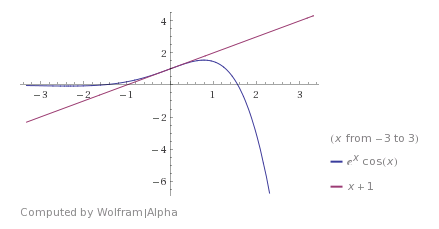
\includegraphics[width=5.5cm]{images/PowerSeriesPlot1.png} \\
     	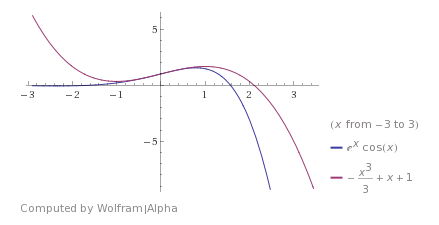
\includegraphics[width=5.5cm]{images/PowerSeriesPlot2.png} 
    	\column{.5\textwidth}
     	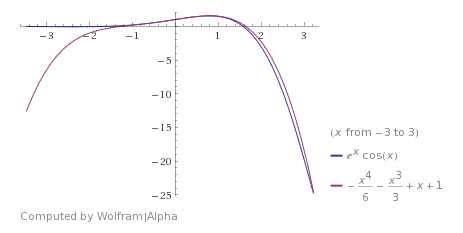
\includegraphics[width=5.5cm]{images/PowerSeriesPlot3.png} \\
     	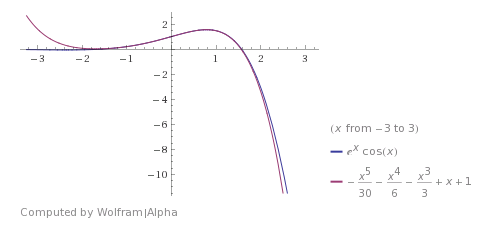
\includegraphics[width=5.5cm]{images/PowerSeriesPlot4.png} 
    	\end{columns}
\end{frame}
  
\begin{frame}{Accuracy of Series Approximations}
\end{frame}
  
\begin{frame}{Some Uses of Series}
\end{frame}

\end{document}
